\documentclass{article}
\usepackage[T1]{fontenc}
\usepackage{lmodern}
\usepackage{graphicx}
\usepackage{amsmath,amssymb}
\usepackage[a4paper,margin=2cm]{geometry}
\usepackage[absolute,overlay]{textpos}
\setlength{\TPHorizModule}{1mm}
\setlength{\TPVertModule}{1mm}
\usepackage[indonesian]{babel}
\usepackage{hyperref}
\setlength{\emergencystretch}{2em}
% unit: Halaman 115

\begin{document}

% === Halaman 115 (llm) ===

\vspace{166.32mm}

\begin{itemize}
    \item Jerman sangat percaya diri bahwa Enigma tidak akan dapat dipecahkan.
    \item Namun, dengan bantuan Polandia, Perancis dan Inggris kemudian membuat mesin pemecah Enigma baru ini, yang diberi nama \textit{bombe}.
    \item \textit{Bombe} dirancang oleh Alan Turing.
    \item \textit{Bombe} berhasil memecahkan Enigma Cipher buatan Jerman.
    \item Keberhasilan memecahkan Enigma Cipher dianggap sebagai faktor yang memperpendek perang dunia kedua menjadi hanya dua tahun.
\end{itemize}

\vspace{10mm}

Coba simulator online Enigma di: \url{https://www.101computing.net/enigma/enigma-instructions.html}

% deskripsi: Foto hitam putih mesin Bombe yang digunakan untuk memecahkan kode Enigma
% bbox normalisasi: [0.6110, 0.0930, 0.9560, 0.6530]
\begin{textblock*}{72.45mm}(128.31mm,27.62mm)
\noindent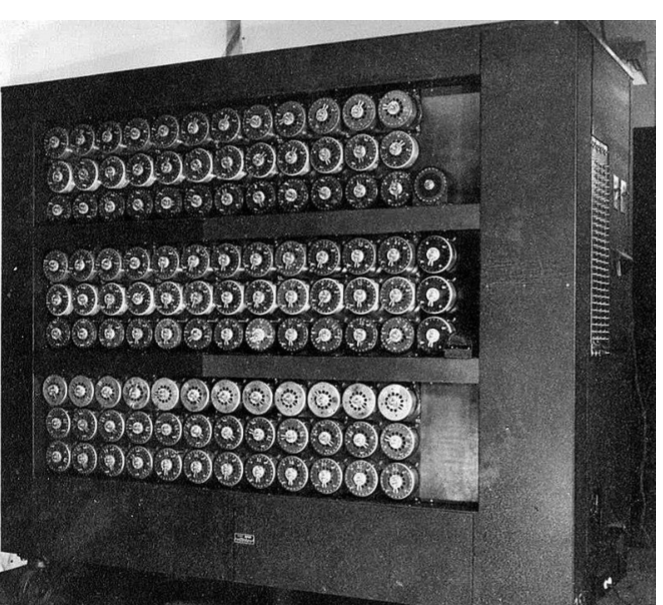
\includegraphics[width=72.45mm,height=166.32mm]{../../images/llm/page_115_img_01.png}%
\end{textblock*}

\end{document}
